\documentclass[12pt,a4paper]{article}
\usepackage[width=.75\textwidth]{caption}
\usepackage{graphicx}
\usepackage{changepage}
\usepackage{authblk}
\usepackage{amsmath}
\usepackage{amsfonts}
\usepackage{amssymb}
\usepackage{braket}
% \usepackage{epigraph}
\usepackage{etoolbox}
\usepackage{orcidlink}
\usepackage[mathscr]{euscript}
\usepackage[top=2cm, bottom=2cm, left=2cm, right=2cm]{geometry}
\usepackage{fancyhdr}
\usepackage{tikz-cd}
\newcommand{\dv}[1]{\mathrm{d} #1 \text{ }}

\newcommand*\diff{\mathop{}\!\mathrm{d}}
% \newcommand\restr[2]{{% we make the whole thing an ordinary symbol
%   \left.\kern-\nulldelimiterspace % automatically resize the bar with \right
%   #1 % the function
%   \vphantom{\big|} % pretend it's a little taller at normal size
%   \right|_{#2} % this is the delimiter
%   }}
% \setlength{\epigraphwidth}{0.8\textwidth}

% \pagestyle{fancy}
\begin{document}

%title and author details
\title{Gravity from Quantum Measurement}
\author[ ]{Kevin Player\footnote{\textit{kjplaye@gmail.com}} \,\orcidlink{0009-0000-7180-7985}}

\maketitle

% \epigraph{The Unruh effect tells us that what we call particles is really just a matter of perspective.}{Lee Smolin}


\abstract{We propose a framework in which gravity can emerge from the physical backreaction of quantum measurement and the microstate dynamics of information acquisition. Standard results, including horizon scales and entropy bounds, follow from Landauer's principle at the Unruh temperature. We then present a concrete bilocal microstate construction as a case-study. Entangled pairs emitted from a localized source propagate into left and right Rindler wedges, where polarization measurement events produce discrete energy-momentum impulses and correlated classical bits. These microstates can be described geometrically using Aichelburg--Sexl pp-wave solutions, whose longitudinal shifts and transverse focusing imprint energy and information directly onto horizon geometry. This setup illustrates how individual measurement events contribute to horizon entropy, and how entanglement can be converted into spatial information, providing an operational realization of ER=EPR at the level of single microstates. The framework complements entropic and thermodynamic approaches by supplying a concrete, microphysical model linking quantum measurement, horizon dynamics, and emergent spacetime.}

\section{Introduction}

Two landmark results establish that gravity and thermodynamics are deeply intertwined. Jacobson showed that the Einstein equations can be derived from thermodynamic identities applied to local Rindler horizons, with horizon entropy playing the role of the fundamental quantity from which spacetime dynamics emerge~\cite{jacobson1995thermodynamics}. Verlinde extended this perspective, arguing that gravitational forces arise from entropy gradients on holographic screens, recasting gravity as an entropic rather than a fundamental interaction~\cite{entropic}. Both frameworks, however, operate at the level of bulk thermodynamics and leave open a prior question: what physical process underlies each individual entropy increment?

We argue that the answer is quantum measurement. Each act of information acquisition by a physical observer constitutes a discrete microstate event, and the collective backreaction of such events---together with the causal correlations they induce---gives rise to gravitational effects. The argument proceeds in three steps. First, any observation is mediated by a physical interaction: information transfer necessarily involves an exchange of energy and momentum between the observed system and the detector, a discrete impulse. Second, by the equivalence principle, this impulse is locally indistinguishable from the effect of a gravitational field: no local measurement can distinguish the recoil associated with a quantum measurement event from free fall in a gravitational potential. Third, when such impulses are modelled geometrically---via Aichelburg--Sexl (AS) pp-wave solutions, as we show---they imprint energy and information directly onto horizon geometry, and coarse-graining over the resulting ensemble recovers standard horizon thermodynamics.

A unifying structure runs through all three of these relations, and it is worth making explicit before proceeding. In each case, the relation between two adjacent concepts has the same logical character: every instance of the more abstract concept is grounded in an instance of the more physical one, but not every instance of the more physical concept gives rise to the more abstract one \emph{for a given observer}. The gap in each case is filled by subjectivity. Quantum state reduction is always backed by an observation---it just is a Bayesian update on the observer's part---but an observation that carries no new information for that observer produces no state reduction. Equally, every observation is backed by an energy-momentum transfer, but not every such transfer constitutes an observation for you: an interaction involving a different observer leaves your state unchanged. The Unruh effect suggests the same structure extends to the equivalence principle: an accelerating observer perceives a thermal bath and attributes it to a gravitational field, while an inertial observer sees only vacuum. Whether an acceleration counts as gravity is perspectival in precisely the same sense. In each case the relation is an identification, not a causal link, and the identification is observer-relative.

This stands in sharp contrast to the Penrose--Di\'osi objective collapse programme~\cite{penrose1996gravity, diosi1987universal}, which postulates that gravity \emph{causes} quantum state reduction as an objective, observer-independent physical process. Figure~\ref{fig:diagram} summarises this contrast. The three solid arrows represent the perspectival grounding relations described above; the single dashed arrow represents the Penrose--Di\'osi causal postulate. It is the only relation in the diagram claimed to be objective and observer-independent, and it is the only one we do not adopt.

\begin{figure}[h]
\centering
\begin{tikzcd}[row sep=4em, column sep=7em]
\text{Gravitational field} \arrow[r, dashed, "\scalebox{0.7}{\shortstack{Penrose--Di\'osi}}"]
    & \text{Quantum state reduction} \\
\text{Acceleration} \arrow[u, "\scalebox{0.7}{\shortstack{equivalence\\principle}}"']
                    \arrow[r, "\scalebox{0.7}{\shortstack{energy--momentum\\transfer}}"']
    & \text{Observation} \arrow[u, "\scalebox{0.7}{\shortstack{Bayesian\\update}}"']
\end{tikzcd}
\caption{Solid arrows denote substrate relations: $A \to B$ means every instance of $B$ is physically realised by an instance of $A$, for a given observer. The dashed arrow denotes the Penrose--Di\'osi postulate, where the relation is claimed to hold objectively rather than observer-relatively.}
\label{fig:diagram}
\end{figure}

To make this concrete, we build on the microstate construction of~\cite{player2025driving}, in which bilocal driving sources generate entangled Rindler excitations that realise individual terms of the Unruh thermal ensemble. The present paper applies and extends that construction. Entangled pairs emitted from a localised source propagate into left and right Rindler wedges; polarisation measurement events produce discrete energy-momentum impulses and correlated classical bits. We show that each such microstate carries a calculable gravitational imprint, modelled by an AS pp-wave solution, and that coarse-graining over the ensemble recovers standard horizon thermodynamics. This construction also provides an operational realisation of ER=EPR at the level of individual microstates: entanglement is converted into geometric information, and each measurement event contributes a discrete, calculable increment to horizon entropy.

This approach both complements and sharpens the thermodynamic gravity programme of Jacobson and Verlinde. Jacobson's derivation of the Einstein equations from horizon thermodynamics and Verlinde's entropic force framework both operate at the level of bulk averages, leaving open the question of what physical process underlies each entropy increment. The present construction supplies that microstate realisation: each entropy increment corresponds to a physically mediated measurement event with a calculable energy-momentum transfer. Thermality is emergent rather than intrinsic, arising from coarse-graining over an ensemble of source-driven microstates, each of which admits a definite, non-thermal description in the global Minkowski frame. The thermodynamic results of both programmes are recovered as a consequence of this coarse-graining, rather than assumed as a starting point.


[Section map paragraph todo]

\section{Motivating Heuristics}
\label{sec:heuristics}

The central observation is simple. Landauer's principle associates a minimal energy cost with the acquisition of information \cite{landauer1961irreversibility}. For an accelerated observer, the relevant temperature is the Unruh temperature \cite{unruh1976notes}. Substituting one into the other eliminates temperature entirely, yielding a frame-independent relation between information acquisition, energy transfer, and acceleration (a version of the BHT first law). This is not merely an algebraic convenience: it is a concrete dictionary between the thermal description natural to a Rindler observer and the non-thermal global Minkowski description, with the apparent thermality of the vacuum emerging as a consequence of the observer's acceleration rather than as a fundamental property of the state. In this way we derive a sequence of standard results in black hole thermodynamics.

\subsection{The Unruh-Landauer Relation}
Landauer's principle states that the acquisition of $\Delta S$ bits of information by a physical observer requires a minimum energy transfer
\begin{equation}
\Delta E \geq k_B T \, \Delta S.
\end{equation}
For an observer undergoing proper acceleration $a$, the Unruh effect associates a temperature
\begin{equation}
T = \frac{\hbar a}{2 \pi k_B c}
\end{equation}
with the local vacuum. Substituting into Landauer's bound eliminates $k_B T$, yielding
\begin{equation}
\boxed{\Delta E \geq \frac{\hbar a}{2\pi c} \, \Delta S.}
\label{eq:UL}
\end{equation}
Temperature has dropped out entirely: equation~\eqref{eq:UL} is a frame-independent relation between energy, acceleration, and information, with no reference to any thermal description. It can be read as the first law of black hole thermodynamics derived from below — from the physical cost of information acquisition — rather than postulated as a thermodynamic identity. In what follows, all standard results emerge as consequences of this single relation.
We note that Landauer's principle is conventionally stated for information erasure rather than acquisition. Here we apply it to acquisition, which is the physically relevant process for an observer registering a measurement outcome. The bound has the same form in both cases; we apply it to acquisition on the grounds that registering a measurement outcome is physically equivalent to a bit being written into the detector's state, which is the process Landauer's principle governs.
\subsection{Momentum Transfer and Acceleration}
The energy transfer $\Delta E$ implied by equation~\eqref{eq:UL} is carried by a physical quantum — matter or radiation — mediating the measurement interaction. We refer to this as the \emph{thrust quantum}. For a relativistic carrier, the associated momentum transfer is
\begin{equation}
\Delta p = \frac{\Delta E}{c}.
\end{equation}
Let the interaction occur over a spatial scale $r$, so that the interaction time is $\Delta t \sim 2r/c$. For a detector of mass $m_d$, Newton's second law in impulse form gives
\begin{equation}
a = \frac{\Delta p}{m_d \Delta t} = \frac{\Delta E}{2 m_d r}.
\label{eq:accel}
\end{equation}
The factor of 2 in the interaction time is not an independent assumption: it will be fixed self-consistently by requiring that the characteristic interaction scale reproduces the Schwarzschild radius, as shown in the next subsection.
\subsection{The Schwarzschild Radius}
The thrust quantum carries energy $\Delta E$ and produces an acceleration $a$ on the detector. Identifying this with the Newtonian gravitational acceleration due to a mass $m_t$ at distance $r$.
\begin{equation}
a = \frac{G m_t}{r^2},
\end{equation}
and substituting equation ~\eqref{eq:accel} with $\Delta E=m_t c^2$, we obtain
\begin{equation}
\frac{m_t c^2}{2 m_d r} = \frac{G m_t}{r^2}.
\end{equation}
Solving for $r$:
\begin{equation}
r = \frac{2 G m_d}{c^2} \equiv r_s,
\end{equation}
which is precisely the Schwarzschild radius of the detector mass $m_d$. This fixes the factor of 2 in the interaction time retroactively: the choice $\Delta r = 2r/c$ is the unique one consistent with Newtonian gravity and the correct Schwarzschild scale.

\subsection{Surface Gravity}
Evaluating the acceleration at $r = r_s$ gives the surface gravity of the detector:
\begin{equation}
\kappa = \frac{G m_d}{r_s^2} = \frac{c^4}{4 G m_d},
\end{equation}
in agreement with the standard Schwarzschild result. This is the acceleration that appears in the Unruh temperature associated with the detector's horizon, $T = \hbar \kappa / 2\pi k_B c$, providing an internal consistency check on the framework.

\subsection{Bekenstein-Hawking Entropy}
Returning to the Unruh-Landauer relation~\eqref{eq:UL} and substituting the surface gravity $\kappa$ for $a$, the entropy increment associated with an energy increment $\Delta E = c^2 \Delta m_d$ is
\begin{equation}
\Delta S \leq \frac{2\pi c}{\hbar \kappa} \Delta E = \frac{8\pi G m_d}{\hbar c^3} \cdot c^2 \Delta m_d.
\end{equation}
Expressing this in terms of the change in Schwarzschild area $\Delta A = 32\pi G^2 m_d \Delta m_d / c^4$:
\begin{equation}
\Delta S \le \frac{\Delta A}{4 \ell_P^2}, \qquad \ell_P^2 = \frac{\hbar G}{c^3},
\end{equation}
which is the Bekenstein-Hawking area law. Each measurement event contributes a discrete entropy increment proportional to the area imprinted on the horizon by the associated energy-momentum transfer.

The two bounds are saturated simultaneously when $a = c^2/R$ — which is exactly the condition for being {\it at a horizon}. The horizon is therefore not just where thermodynamics happens to work out, it is the unique locus where the minimum cost of information acquisition equals the maximum information content of the region.

\subsection{Summary}
Beginning from the single relation~\eqref{eq:UL}, and using only Newton's law and the equivalence principle, we have recovered the Schwarzschild radius, the surface gravity, and the Bekenstein-Hawking area law as consequences of the observation=acceleration identification. These are standard results, but their derivation here from the physical cost of information acquisition rather than from thermodynamic postulates is the point. The thrust quantum introduced in this section — the physical carrier of the measurement-induced impulse — will be given a precise microstate realization in the sections that follow, where it is identified with an individual photon modeled as an Aichelburg-Sexl pp-wave.


\section{Bilocal Microstate Construction}
\label{sec:microstates}

The heuristic arguments of Section~\ref{sec:heuristics} establish a relationship between
information acquisition, acceleration, and gravitational effects, but leave open the question
of what a single microstate looks like concretely. In standard treatments, the Unruh effect
is derived by coupling a detector to a pre-existing acceleration and reading off a thermal
response from the vacuum. Following~\cite{player2025driving}, we invert this logic: we place
an interaction in the past, where a source injects non-thermal entangled excitations into the
field, and show that the observer's accelerated response is driven by these source-induced
excitations. The thermal ensemble then emerges as a coarse-grained aggregate of such
microstates, rather than being a primitive property of the vacuum.

We now upgrade this construction from a spin-0 scalar field to the spin-1 electromagnetic
field. This is not merely a technical generalisation. As we show, the photon carries a unit
of action $\hbar$ per cycle alongside its energy $E = \hbar\omega$, which closes the
Landauer gap left open in Section~\ref{sec:heuristics}: the minimum actionable event in the
construction is precisely a single photon, and its polarisation state constitutes the
classical bit acquired by each observer. The anticorrelated helicities of the entangled pair
are the natural completion of the $\mathbb{Z}_2$ swap symmetry between wedges, and as we
discuss in Section~\ref{sec:ppwave}, they imprint a definite geometric signature onto the
horizon consistent with the ER=EPR identification.

%------------------------------------------------------
\subsection{The Paz--Lester--Wright Setup}
%------------------------------------------------------

We retain the Alice-and-Bob style naming convention. Three observers are placed at spacetime
positions $(t,z) = (0,1)$, $(0,-1)$, and $(-1,0)$, named \emph{Wright}~(R), \emph{Lester}~(L),
and \emph{Paz}~(P) respectively --- a mnemonic for Right, Left, and Past. Paz serves as the
common causal ancestor of Wright and Lester (see Figure~\ref{paz}).

\begin{figure}[h]
\centering
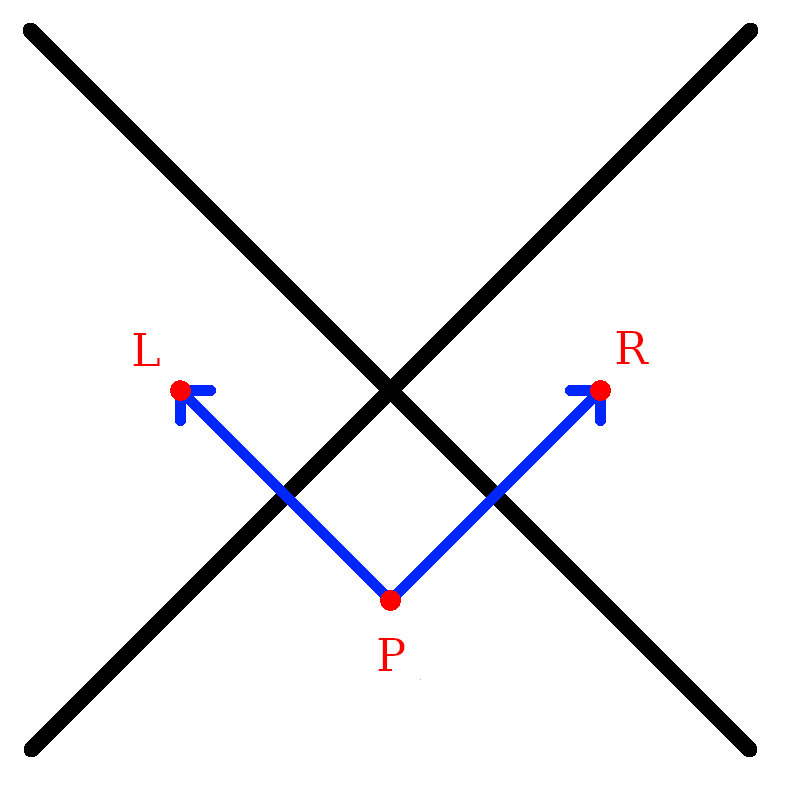
\includegraphics[scale=0.75]{paz.png}
\captionsetup{width=0.7\textwidth}
\caption{A source in the past, Paz~(P), emits an entangled photon pair that accelerates
Wright~(R) into the right Rindler wedge and Lester~(L) into the left Rindler wedge.
The two null directions of propagation define the $x^+$ and $x^-$ axes of the double-null
coordinate system.}
\label{paz}
\end{figure}

Paz emits an entangled pair of spin-1 massless photons with momenta $\pm k$ and Rindler
frequency $\omega = \omega_k$. The momenta are perfectly balanced, so the source exhibits no
net back-reaction in this minimal model --- a simplification discussed further in
Section~\ref{sec:drive_phy}. The two photons propagate into the left and right Rindler wedges,
where Lester and Wright detect them respectively, each registering a helicity eigenvalue and
acquiring one classical bit of information.

%------------------------------------------------------
\subsection{Double-Null Gauge}
%------------------------------------------------------

The emission event naturally defines two null directions: the right-moving photon has
wave-vector $k^\mu_R$ and the left-moving photon has wave-vector $k^\mu_L = -k^\mu_R$. These
two null directions are precisely the $x^+$ and $x^-$ axes of double-null coordinates
\begin{equation}
    x^\pm = \frac{1}{\sqrt{2}}(t \pm z),
\end{equation}
with transverse coordinates $\mathbf{x}_\perp = (x^1, x^2)$. Working in this frame we impose
the symmetric double-null gauge condition
\begin{equation}
    A_+(x) = 0, \qquad A_-(x) = 0,
\label{eq:doublenull}
\end{equation}
so that the gauge field is supported entirely on the transverse components
$\mathbf{A}_\perp = (A^1, A^2)$. This gauge respects the $\mathbb{Z}_2$ symmetry that swaps
the two wedges $(x^+ \leftrightarrow x^-)$ simultaneously with $(R \leftrightarrow L)$, and
therefore treats both observers symmetrically by construction. The residual gauge freedom is
fixed by requiring $\partial_i A^i = 0$ in the transverse plane, leaving precisely the two
physical helicity degrees of freedom $\epsilon^i_{(\lambda)}$ with $\lambda = \pm 1$.

The lack of manifest four-dimensional covariance in~\eqref{eq:doublenull} is a consequence
of aligning the gauge with the pair of physical null directions selected by the source, rather
than an arbitrary choice. The full Lorentz group is broken to the little group preserving the
pair $\{k^\mu_R, k^\mu_L\}$, which is the two-dimensional Euclidean group $ISO(2)$ acting on
the transverse plane. This is precisely the little group of massless particles, and the two
helicity eigenstates $\lambda = \pm 1$ are its irreducible representations. All physical
results are independent of the gauge choice.

%------------------------------------------------------
\subsection{The Bilocal Source}
%------------------------------------------------------

In double-null gauge the electromagnetic field is characterised by its transverse components
alone. The bilocal driving source generalises the scalar construction to
\begin{equation}
    J^{ij}(x,y) = \lambda\; \epsilon^{i*}_{(-1)}\, \epsilon^{j}_{(+1)}\; f_L(x)\, f_R(y),
\label{eq:bilocal_vec}
\end{equation}
where $\lambda$ is a coupling constant, $f_L$ and $f_R$ are normalised mode profiles supported
on the left and right wedges respectively, and $\epsilon^i_{(\lambda)}$ are the circular
polarisation vectors
\begin{equation}
    \epsilon^i_{(+1)} = \frac{1}{\sqrt{2}}\begin{pmatrix}1\\i\end{pmatrix}, \qquad
    \epsilon^i_{(-1)} = \frac{1}{\sqrt{2}}\begin{pmatrix}1\\-i\end{pmatrix}.
\end{equation}
The index structure of~\eqref{eq:bilocal_vec} assigns helicity $+1$ to the right-moving mode
and helicity $-1$ to the left-moving mode: the pair is \emph{anticorrelated} in helicity. This
is the unique assignment consistent with angular momentum conservation at the emission vertex
and with the $\mathbb{Z}_2$ wedge-swap symmetry, under which $\epsilon^i_{(+1)} \leftrightarrow
\epsilon^i_{(-1)}$.

The sourced Lagrangian reads
\begin{equation}
\begin{aligned}
    \mathscr{L}_{\text{sourced}}
    &= \mathscr{L}_{\text{free}}
      + \tfrac{1}{2}\lambda \int
          J^{ij}(x,y)\; A^+_i(x)\, A^+_j(y)\; d^4x\, d^4y
      \;+\; \text{h.c.} \\
    &= \mathscr{L}_{\text{free}}
      + \tfrac{1}{2}\lambda
        \Bigl(
          a^{L\dagger}_{-k,(-1)}\, a^{R\dagger}_{k,(+1)}
          \;+\;
          a^{L}_{-k,(-1)}\, a^{R}_{k,(+1)}
        \Bigr),
\end{aligned}
\label{eq:bilocal_lag}
\end{equation}
where $a^{L\dagger}_{-k,(-1)}$ and $a^{R\dagger}_{k,(+1)}$ are creation operators for
left-wedge helicity $-1$ and right-wedge helicity $+1$ modes respectively. The interaction
term in~\eqref{eq:bilocal_lag} is a two-mode squeezing interaction at frequency $\omega$,
now resolved by helicity: it is the direct vector-field analogue of the scalar squeezing
interaction~\cite{gerry2023introductory}, with the anticorrelated polarisation structure
made explicit. The photon pair carries total angular momentum zero, consistent with emission
from a scalar source at Paz.

Each photon carries energy $E = \hbar\omega$ and, as a mode of the electromagnetic field,
constitutes precisely one quantum of action $\hbar$ per oscillation cycle. The thrust quantum
of Section~\ref{sec:heuristics} is thereby identified with a single photon: the minimum
actionable event is the emission and detection of one such quantum. The energy transferred
per bit acquired is $\Delta E = \hbar\omega$, saturating the Unruh--Landauer bound~\eqref{eq:UL}
at the fundamental quantum level. This closes the Landauer gap: registering a photon's
helicity writes one classical bit into the detector's physical state, which is precisely the
process Landauer's principle governs.

%------------------------------------------------------
\subsection{Polarisation Bogoliubov Transformation}
%------------------------------------------------------

We now show that the polarisation labels survive the Rindler--Unruh mode decomposition,
so that the thermal ensemble retains its helicity structure and the anticorrelation of the
emitted pair descends unambiguously to the level of individual Rindler microstates.

In the transverse plane, the electromagnetic field in double-null gauge decomposes into
two independent scalar-like sectors labelled by helicity $\lambda = \pm 1$. For each sector,
the right-wedge field expands as
\begin{equation}
    A^i_\lambda(x) = \int_0^\infty \frac{d\Omega}{2\pi}\,
        \frac{1}{\sqrt{2\Omega}}\,\epsilon^i_{(\lambda)}
        \left[
            b^R_{\Omega,\lambda}\, u^R_\Omega(x)
            + b^{R\dagger}_{\Omega,\lambda}\, u^{R*}_\Omega(x)
        \right],
\end{equation}
where $u^R_\Omega(x)$ are the right-wedge Rindler modes at Rindler frequency $\Omega$, and
$b^R_{\Omega,\lambda}$, $b^{R\dagger}_{\Omega,\lambda}$ are the corresponding annihilation
and creation operators satisfying
\begin{equation}
    \left[b^R_{\Omega,\lambda},\, b^{R\dagger}_{\Omega',\lambda'}\right]
    = \delta(\Omega - \Omega')\,\delta_{\lambda\lambda'}.
\end{equation}
An identical expansion holds in the left wedge with $R \to L$ and $\lambda \to -\lambda$,
reflecting the anticorrelated helicity assignment. Because each helicity sector is
independently a scalar-like sector, the Bogoliubov transformation relating Minkowski and
Rindler modes takes the same form in each sector. For helicity $\lambda$ at Rindler
frequency $\Omega$, the Unruh modes are
\begin{equation}
    c_{\Omega,\lambda} = \cosh\theta_\Omega\; b^R_{\Omega,\lambda}
                       - \sinh\theta_\Omega\; b^{L\dagger}_{\Omega,-\lambda},
\label{eq:bogoliubov}
\end{equation}
where $\tanh\theta_\Omega = e^{-\pi\Omega c/a}$ encodes the Unruh distribution at
acceleration $a$, and $-\lambda$ on the left-wedge operator reflects the anticorrelation.
The transformation~\eqref{eq:bogoliubov} is the standard Bogoliubov relation for a massless
field~\cite{unruh1976notes, birrell1982quantum}, now carrying a helicity label throughout.
The Minkowski vacuum in the Rindler basis reads, for each helicity sector,
\begin{equation}
    |0\rangle_M^{(\lambda)}
    = \frac{1}{\cosh\theta_\Omega}
      \sum_{n=0}^\infty \tanh^n\theta_\Omega\;
      |n_{\Omega,\lambda}\rangle_R\,
      |n_{\Omega,-\lambda}\rangle_L,
\label{eq:vacuum_vec}
\end{equation}
and the full vacuum is the product over all $\Omega$ and both helicities:
\begin{equation}
    |0\rangle_M = \prod_{\Omega,\lambda} |0\rangle_M^{(\lambda)}.
\end{equation}

Equation~\eqref{eq:vacuum_vec} makes explicit that the Minkowski vacuum is a sum over
entangled helicity-anticorrelated pairs at each Rindler frequency. The bilocal source
selects a single term from this sum at fixed $\Omega$ and fixed helicity pair
$(\lambda, -\lambda) = (+1,-1)$, yielding the single-microstate
\begin{equation}
    |\Psi_{\Omega}\rangle_M
    = |1_{\Omega,+1}\rangle_R\,|1_{\Omega,-1}\rangle_L
      + \mathcal{O}(\text{higher order}).
\label{eq:microstate_vec}
\end{equation}
Wright's detection of helicity $+1$ and Lester's detection of helicity $-1$ are therefore
perfectly anticorrelated: each measurement event yields one classical bit, and the two bits
are the complement of one another. Table~\ref{table:modes} summarises the correspondence
between mode profiles, operators, helicity labels, and states.

The key structural result is that the helicity label $\lambda$ is conserved under the
Bogoliubov transformation: it enters equation~\eqref{eq:bogoliubov} as a spectator index and
exits unchanged on the Unruh operators $c_{\Omega,\lambda}$. Thermality, when it arises from
coarse-graining over the ensemble of microstates~\eqref{eq:microstate_vec}, is therefore
helicity-resolved: each helicity sector thermalises independently, and the anticorrelation
between wedges is preserved at every level of the construction.

%------------------------------------------------------
\subsection{Summary of the Vector Upgrade}
%------------------------------------------------------

The passage from the scalar to the vector field construction introduces three structural
improvements. First, the photon carrying $E = \hbar\omega$ and one quantum of action per
cycle identifies the thrust quantum of Section~\ref{sec:heuristics} with a concrete physical
object, closing the Landauer acquisition gap. Second, the double-null gauge condition,
motivated by the pair of null directions defined by the emission event, treats both Rindler
wedges symmetrically and exposes the $\mathbb{Z}_2$ swap symmetry as the organising principle
of the construction. Third, the anticorrelated helicity structure, conserved through the
Bogoliubov transformation, provides each observer with one classical bit whose values are
perfectly complementary: the two bits together constitute the correlated classical record
that, in the AS pp-wave picture of Section~\ref{sec:ppwave}, is imprinted as geometric
information onto the horizon.

\subsection{Matter as Substrate: Ticks, Memory, and the Thrust Quantum}
\label{sec:substrate}

The claim that information is encoded in matter and energy rather than in the horizon
geometry requires a physical account of what it means for matter to \emph{carry} information.
We outline that account here, drawing on the matter channel picture of~\cite{player2025matter}.

A massive particle accumulates phase along its worldline at a rate set by its rest energy.
The De Broglie relation $f = E/h$ assigns a natural frequency to any mass $m$, and
Bremermann's computational limit independently recovers the same rate $f_{Br} = mc^2/h$ as
the maximum clock rate of any physical system with that energy~\cite{bremermann1962optimization}.
These two results agree because they are both expressions of the same underlying fact: a
quantum of action $\hbar$ is the minimal unit of physical evolution, and $mc^2/h$ is the
rate at which a mass $m$ consumes such quanta. Each such quantum corresponds to one tick of
the phase $e^{iS/\hbar}$ in the path integral, and classical trajectories emerge from the
constructive interference of these ticks across paths.

This gives matter a precise sense in which it is a \emph{substrate for information}: it
accumulates ticks, and each tick is a discrete, Lorentz-invariant event recorded in the
particle's proper time. Matter is persistent memory in the operational sense that its history
of ticks is physically encoded in its state and cannot be erased without an energy cost
governed by Landauer's principle. The maximum rate of this memory is bounded by Bremermann;
the maximum total capacity is bounded by the Bekenstein bound, which we have already derived
in Section~\ref{sec:heuristics} as a consequence of the Unruh--Landauer relation rather than
as an independent postulate.

A massless particle --- the photon --- has no rest frame, no proper time, and accumulates no
action between emission and absorption. It does not tick. It therefore carries no persistent
memory and cannot serve as a substrate. Its role in the present construction is precisely
that of a pure information carrier. A single photon carries exactly two irreducible
constituents, distinct in kind:
\begin{itemize}
    \item \textbf{One quantum of action $\hbar$}: the physical transfer, deposited into the
    detector's matter-memory as one additional tick. This is what makes the interaction
    irreversible and imposes the Landauer energy cost.
    \item \textbf{One bit of polarisation}: the informational outcome, the classical record
    of which helicity --- $\lambda = +1$ or $\lambda = -1$ --- was absorbed. This is what
    is correlated between Wright and Lester and constitutes the spatial bit of
    Section~\ref{sec:erepr}.
\end{itemize}
These are not the same thing in different guises. The $\hbar$ is what makes the event
physical; the bit is what makes it meaningful to an observer. That a single photon carries
exactly one of each is not a coincidence: it is why the photon is the natural minimal unit
of the entire construction, the unique object that saturates both the action and the
information count simultaneously. The energy deposited is $\Delta E = \hbar\omega$,
saturating the Unruh--Landauer bound at the fundamental quantum level, as established in
Section~\ref{sec:microstates}.

The horizon enters this picture not as a storage medium but as a boundary condition. It marks
the surface at which the matter-memory on one side is causally disconnected from the
matter-memory on the other. Horizon entropy, in this account, is not a property of the
horizon surface itself but a count of the ticks that have been written into the matter on
each side --- bounded by Bremermann from above and by Landauer from below. The holographic
appearance of this count, proportional to area rather than volume, is a consequence of the
Unruh--Landauer and Bekenstein relations derived in Section~\ref{sec:heuristics} and does not
require holography as an independent postulate.

This reframing has a direct consequence for the ER=EPR identification developed in the
next subsection. The correlated measurement outcomes of Wright and Lester are not encoded
in the horizon geometry in the first instance --- they are encoded in the matter of their
respective detectors, each of which has absorbed one photon and accumulated one additional
tick. The geometric correlations between the two wedges, realised as correlated AS pp-wave
imprints in Section~\ref{sec:ppwave}, are downstream of this matter-level encoding. The
bridge, if it exists, is built from correlated ticks, not from the horizon itself.

\subsection{Matter as Substrate: Ticks, Memory, and the Thrust Quantum - OLD}
\label{sec:substrate}

The claim that information is encoded in matter and energy rather than in the horizon
geometry requires a physical account of what it means for matter to \emph{carry} information.
We outline that account here, drawing on the matter channel picture of~\cite{player2025matter}.

A massive particle accumulates phase along its worldline at a rate set by its rest energy.
The De Broglie relation $f = E/h$ assigns a natural frequency to any mass $m$, and
Bremermann's computational limit independently recovers the same rate $f_{Br} = mc^2/h$ as
the maximum clock rate of any physical system with that energy~\cite{bremermann1962optimization}.
These two results agree because they are both expressions of the same underlying fact: a
quantum of action $\hbar$ is the minimal unit of physical evolution, and $mc^2/h$ is the
rate at which a mass $m$ consumes such quanta. Each such quantum corresponds to one tick of
the phase $e^{iS/\hbar}$ in the path integral, and classical trajectories emerge from the
constructive interference of these ticks across paths.

This gives matter a precise sense in which it is a \emph{substrate for information}: it
accumulates ticks, and each tick is a discrete, Lorentz-invariant event recorded in the
particle's proper time. Matter is persistent memory in the operational sense that its history
of ticks is physically encoded in its state and cannot be erased without an energy cost
governed by Landauer's principle. The maximum rate of this memory is bounded by Bremermann;
the maximum total capacity is bounded by the Bekenstein bound, which we have already derived
in Section~\ref{sec:heuristics} as a consequence of the Unruh--Landauer relation rather than
as an independent postulate.

A massless particle --- the photon --- has no rest frame, no proper time, and accumulates no
action between emission and absorption. It does not tick. It therefore carries no persistent
memory and cannot serve as a substrate. Its role in the present construction is precisely
that of a pure information carrier: the thrust quantum transfers one quantum of action $\hbar$
from Paz's emission event to Wright's or Lester's detection event, writing one tick into
the detector's matter-memory and registering one classical bit. The energy deposited is
$\Delta E = \hbar\omega$, saturating the Unruh--Landauer bound at the fundamental quantum
level, as established in Section~\ref{sec:microstates}.

The horizon enters this picture not as a storage medium but as a boundary condition. It marks
the surface at which the matter-memory on one side is causally disconnected from the
matter-memory on the other. Horizon entropy, in this account, is not a property of the
horizon surface itself but a count of the ticks that have been written into the matter on
each side --- bounded by Bremermann from above and by Landauer from below. The holographic
appearance of this count, proportional to area rather than volume, is a consequence of the
Unruh--Landauer and Bekenstein relations derived in Section~\ref{sec:heuristics} and does not
require holography as an independent postulate.

This reframing has a direct consequence for the ER=EPR identification developed in the
next subsection. The correlated measurement outcomes of Wright and Lester are not encoded
in the horizon geometry in the first instance --- they are encoded in the matter of their
respective detectors, each of which has absorbed one photon and accumulated one additional
tick. The geometric correlations between the two wedges, realised as correlated AS pp-wave
imprints in Section~\ref{sec:ppwave}, are downstream of this matter-level encoding. The
bridge, if it exists, is built from correlated ticks, not from the horizon itself.

\subsection{Entanglement as Spatial Information: ER=EPR at the Microstate Level}

Each measurement produces a polarisation outcome --- $H$ or $V$ --- at each wedge, perfectly
anticorrelated between Lester and Wright. But consider a different question: not \emph{what}
was observed, but \emph{where}. The question ``who observed $H$?'' has a binary answer:
Lester (left wedge) or Wright (right wedge). This is a \emph{spatial bit} --- a bit that
encodes not a polarisation state but a location in space.

The entangled pair has therefore produced classical spatial information --- a left/right
correlation --- from what began as quantum polarisation entanglement. We resist saying the
pair has \emph{converted} one into the other, because the measurement event that reveals the
spatial bit also destroys the entanglement; the precise relationship between the quantum
correlations before measurement and the classical spatial record after it requires more care
than the word ``conversion'' implies.

% TODO: Develop the relationship between entanglement destruction and classical spatial
% record production more carefully. Is there a sense in which the spatial bit is a
% remnant or projection of the pre-measurement entanglement, rather than a conversion of it?
% Relevant literature: Susskind--Maldacena ER=EPR original, Van Raamsdonk entanglement and
% geometry, Papadodimas--Raju interior reconstruction. The question is whether the
% classical bit can be said to *realise* the geometric correlation rather than merely
% *record* it.

What carries the spatial information is not the horizon itself but the \emph{matter and
energy} involved in the measurement events: the photon absorbed by Wright deposits
energy-momentum in the right wedge, and the photon absorbed by Lester deposits
energy-momentum in the left wedge. The horizon is a boundary --- the causal surface
separating the two wedges --- and the information is encoded in the physical degrees of
freedom on either side of it. The horizon's role is to make the left/right distinction
sharp, not to serve as the medium in which information is stored.

% TODO: Develop the matter/energy-as-substrate argument more fully. The heuristics section
% has already replaced the holographic principle with the Unruh--Landauer relation, so the
% argument here should be consistent with that: information is carried by physical quanta
% (thrust quanta / photons), and the holographic counting of horizon microstates is a
% consequence of counting those quanta, not an independent postulate. This subsection
% should eventually make that chain explicit.

This reframing sharpens the ER=EPR identification. The two wedges are connected not by
the horizon as an abstract geometric object but by the physical correlations between the
energy-momentum impulses deposited on each side. In the AS pp-wave picture developed in
Section~\ref{sec:ppwave}, each such impulse produces a measurable longitudinal shift and
transverse focusing of the horizon geometry. The correlated pair of impulses --- one in each
wedge --- produces correlated geometric deformations on the two sides of the horizon,
and it is \emph{this} geometric correlation that constitutes the Einstein--Rosen bridge at
the level of a single microstate.

The spatial bit --- the answer to ``who observed $H$?'' --- is therefore not merely a
record of which side the photon landed on. It is a label for which of the two correlated
geometric deformations was realised, and the two labels together reconstruct the bridge.
This is an operational realisation of ER=EPR at the level of individual microstates:
the entanglement between Lester and Wright's outcomes is not a stand-in for the bridge
but is physically instantiated in the pair of correlated energy-momentum transfers whose
geometric imprint \emph{is} the bridge.

% TODO: Check whether the anticorrelated helicity structure adds anything to the ER=EPR
% identification beyond what the scalar case provides. Helicity is a topological charge
% in 2+1 dimensions (the transverse plane); it is possible that the opposite helicities
% on the two sides contribute a topological twist to the bridge geometry. This would be
% a new result if it can be made precise.



\section{Gravitational Imprint: the pp-Wave Realisation}
\label{sec:ppwave}

Each measurement event in the bilocal construction involves a photon transferring energy and momentum to an accelerated detector. We now model the gravitational imprint of this transfer by identifying each photon with an Aichelburg--Sexl (AS) pp-wave solution in general relativity~\cite{aichelburg1971gravitational}. The AS geometry is an exact solution describing the gravitational field of an ultrarelativistic point mass, and provides the natural geometric language for a single-photon microstate.

\subsection{The AS pp-Wave and Its Effects}

Let $u = t - z$ and $v = t + z$, where the photon propagates along the null plane $u = 0$, $z$ is the longitudinal direction, and $(x,y)$ are transverse coordinates. Test particles at fixed transverse positions $(x,y)$ experience two effects as the shock front crosses $u = 0$:

\begin{enumerate}
    \item \textbf{Longitudinal shift.} The $v$ coordinate is displaced by
    \begin{equation}
    \Delta v \propto -\ln r^2, \qquad r^2 = x^2 + y^2.
    \end{equation}
    This shift is lightlike: no proper time elapses for a particle crossing the shock, but it is displaced along the null direction. Near the axis ($r \to 0$) the shift diverges, encoding the concentration of energy along the photon's trajectory.

    \item \textbf{Transverse focusing.} The gradient of the longitudinal shift produces a transverse velocity
    \begin{equation}
    \Delta \mathbf{v}_\perp \propto \nabla \ln r \propto \frac{1}{r},
    \end{equation}
    directed toward the axis. Test particles are pulled toward the centre of the wave, regardless of their initial transverse separation.
\end{enumerate}

\subsection{The Longitudinal Shift Makes Space}

The longitudinal shift deserves closer attention, because it carries a meaning beyond a mere coordinate displacement. The photon emitted by Paz propagates along the null direction; as it crosses the Rindler horizon, the AS shift displaces the future light cone of every test particle it passes. For the photon traveling into the right wedge, the shift pushes the right wedge's geometry in the $+v$ direction; for the entangled partner traveling into the left wedge, the shift pushes the left wedge in the $-v$ direction. The two wedges are displaced \emph{away from each other} along the longitudinal null direction.

This is not merely a kinematic effect. The transverse plane of the pp-wave is identified with horizon area elements $dA = dx\,dy$, and the longitudinal shift creates a new null interval between the two wedges --- a region of spacetime that did not exist, in the sense of being causally accessible, before the photon passed. The bit of spatial information encoded in the left/right measurement outcome --- ``who observed $H$?'' --- refers to precisely this separation. The measurement event does not merely \emph{record} a spatial distinction; through the gravitational backreaction of the photon, it \emph{creates} the spatial separation that the bit describes.

Put differently: the same physical event --- a photon crossing a horizon --- simultaneously encodes a classical bit and, via the AS longitudinal shift, generates the spatial structure that bit refers to. Space is not a pre-existing backdrop onto which information is written; it is produced, increment by increment, by the gravitational imprint of each measurement event. This is the microstate-level content of emergent space: each detection event contributes both an entropy increment and a spatial increment, and the two are the same thing described in different languages.

\subsection{Horizon Entropy from Individual Microstates}

Each detection event contributes a discrete entropy increment via the Bekenstein--Hawking relation derived in Section~\ref{sec:heuristics}:
\begin{equation}
\Delta S = \frac{\Delta A}{4\ell_P^2}, \qquad \ell_P^2 = \frac{\hbar G}{c^3},
\end{equation}
where $\Delta A$ is the area element imprinted on the horizon by the transverse focusing of the pp-wave. Horizon entropy is therefore not a bulk thermodynamic quantity assigned to the horizon as a whole, but a sum of discrete, calculable contributions from individual measurement-induced interactions. The transverse focusing and the longitudinal shift are two aspects of the same microstate: focusing encodes the entropy increment in the area; the longitudinal shift encodes the spatial increment in the geometry.

\subsection{Coarse-Graining and the Emergence of Thermality}

In a steady-state scenario, Paz continuously emits entangled pairs, and Lester and Wright continuously detect them. Each detection is an AS pp-wave microstate with a definite, non-thermal description in the global Minkowski frame: a specific photon energy, a specific transverse position, a specific longitudinal shift. Coarse-graining over this ensemble recovers the Unruh thermal spectrum at temperature $T = a/2\pi$, consistent with the vacuum decomposition of equation~\eqref{eq:vacuum}. The thermodynamic description of the horizon emerges from this averaging; it is not a feature of the individual microstates.

This completes the microstate programme. Each entropy increment in the Bekenstein--Hawking area law corresponds to a single AS pp-wave interaction. Each pp-wave interaction corresponds to a single measurement event in the bilocal construction. Each measurement event both encodes a spatial bit and generates the spatial separation that bit refers to. The gravitational, thermodynamic, information-theoretic, and geometric descriptions of the horizon are unified at the level of individual microstates, and thermality, entropy, and space itself emerge together from the coarse-grained aggregate of these events.


\section{Conclusion}
\section{Acknowledgements}

I'm also grateful to Claude and ChatGPT for helpful discussions.

\bibliographystyle{ieeetr}
\bibliography{bibliography}

\end{document}
